\documentclass[a4paper]{article}

\hoffset=-1in
\voffset=-1in
\textwidth=175mm
\textheight=250mm

\usepackage{amsmath}
\usepackage{graphicx}
\usepackage{multicol}

\begin{document}
    \begin{figure}
        \centering
        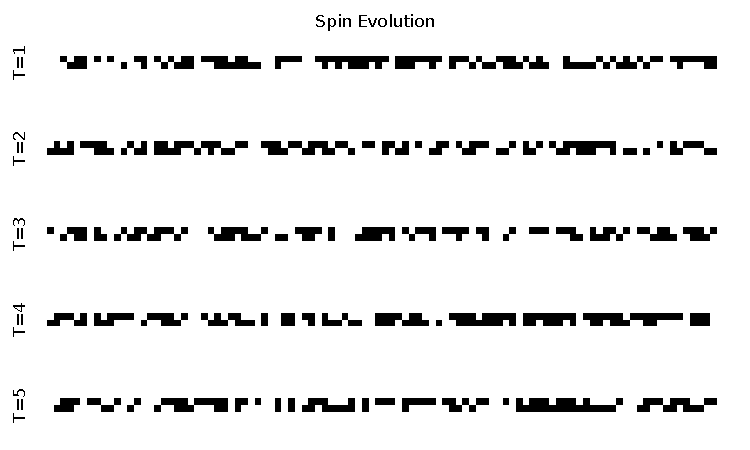
\includegraphics[width=0.8\textwidth]{pub/figures/q1a.pdf}
        \caption{At low temperatures we observed smaller groups of aligned %
            spins. We concluded that the influence of the heat (i.e. %
            \(\tau\sigma\)) on the free energy was low and therefore, that %
            the energy \(U\) was minmised.}
        \label{FIG1}
    \end{figure}

    \begin{figure}  
        \centering
        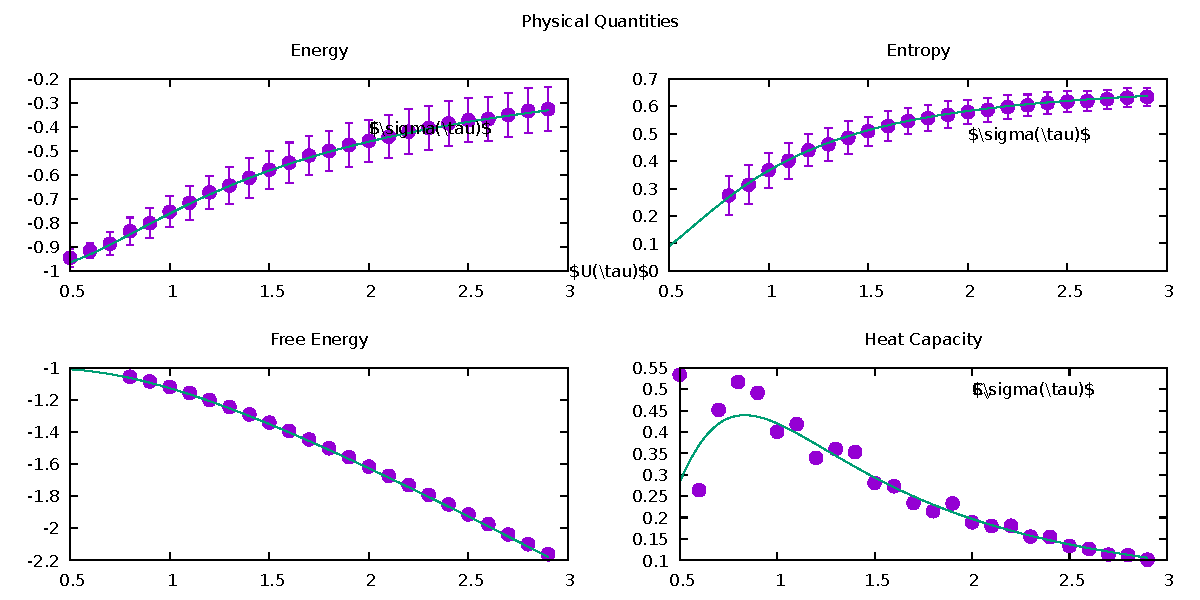
\includegraphics[width=0.8\textwidth]{pub/figures/q1c.pdf}
        \caption{Physical properties of the one-dimensional ising simulation. %
            These figures were generated with 100 repeats at each temperature %
            where one repeat performed 100000 metropolis steps. We noticed %
            the energy, entropy and free energy tended to converge faster than %
            the heat capacity, shown by the relatively large noise. Because, %
            the heat capcity is a function of the variance of the energy %
            we were not able to calculate useful uncertainties in this %
            set of simulations, but based on the larger convergence time we %
            belive they would be large. As expected the variance in the energy %
            was smaller at lower temperatures and increased with the %
            temperature. This makes sense because at low temperature the %
            energy is the factor towards minimising the free energy but at %
            high temperature it is the entropy. Flipping a single spin has %
            a larger affect on the entropy than on the energy explaining this %
            trend in the variance, which remained roughly constant through %
            the second half of the sampled temperatures.}
        \label{FIG2}
    \end{figure}

    \begin{figure}
        \centering
        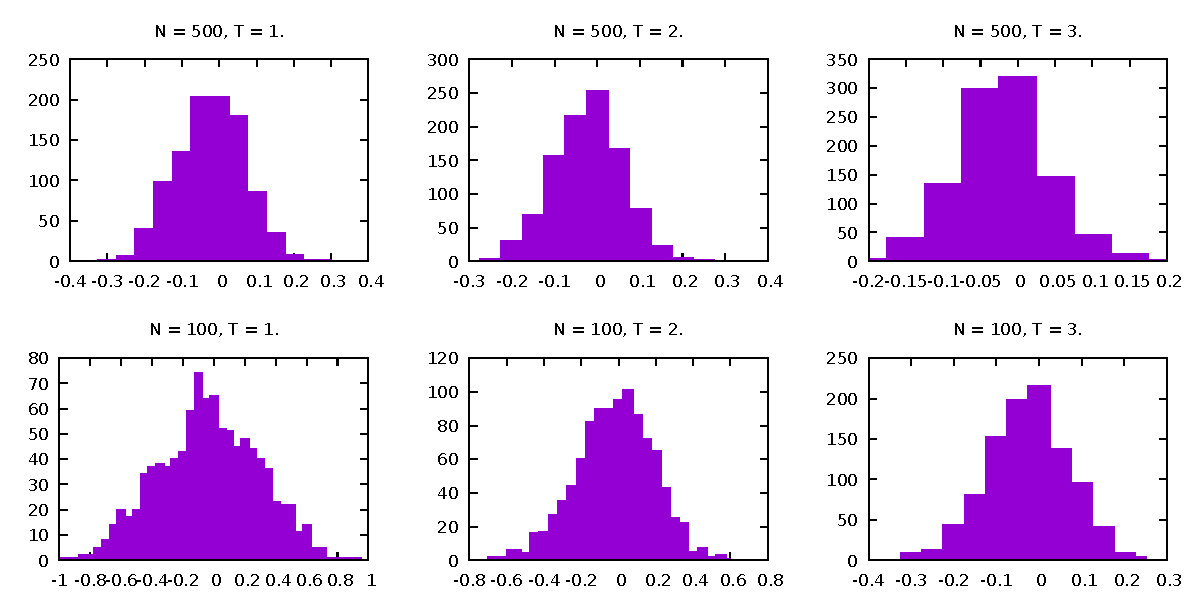
\includegraphics[width=0.8\textwidth]{pub/figures/q1e.pdf}
        \caption{Histograms of the magnetisation per spin as a function of %
            \(N\) and \(T\). We noticed that the magnetisation remained %   
            symmetric around zero for all the temperatures and sizes that we %
            sampled. This makes sense because in the abscence of an external %
            magnetic field there should be no preference for the spins to %
            align in either direction except for that imposed by the %
            interactions between neighbours. We noticed that the distributions %
            were approximately gaussian and that their standard deviations %
            were a decresing function of the temperature. We also noticed %
            that the standard deviation of the system was an increasing %   
            function of the number of spins. Because there was no shift of %
            the magnetisation away from the zero value we concluded that %
            the infinite ising model would become very flat at low %
            temperatures but would not undergo a phase shift, i.e. spontaneous %
            magnetisation.}
        \ref{FIG3}
    \end{figure}
    
    \begin{figure}
        \centering
        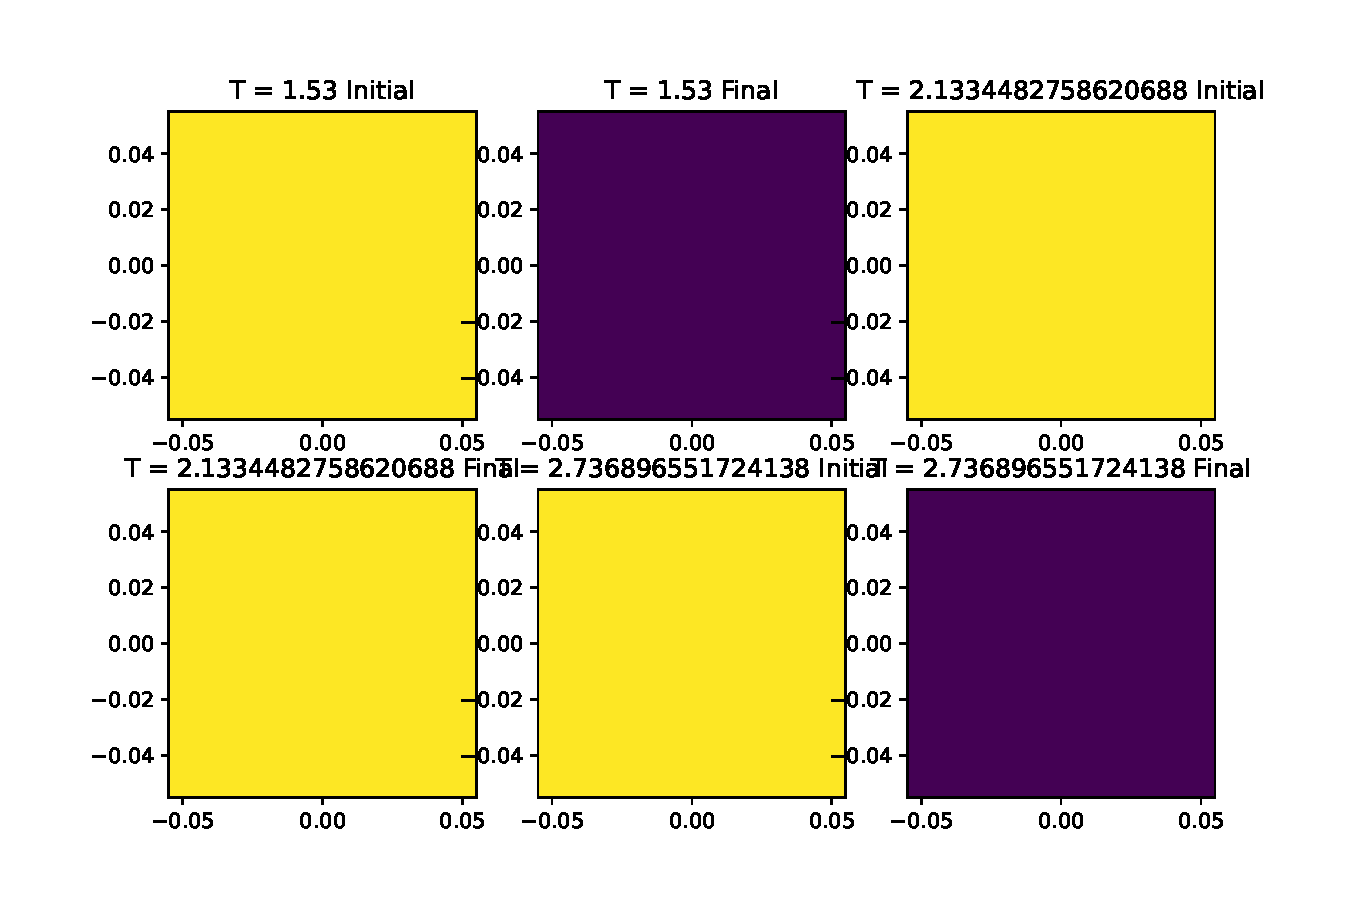
\includegraphics[width=0.8\textwidth]{pub/figures/q2a.pdf}
        \caption{The initial and final states of our two-dimensional ising %
            model simulations. We noticed that at lower temperatures the %
            chunks of aligned spins increased in size. We concluded that %
            the process behind this was a generalisation of the description %
            we gave in the caption to Figure \ref{FIG1}.}
        \label{FIG4}
    \end{figure}

    \begin{figure}
        \centering
        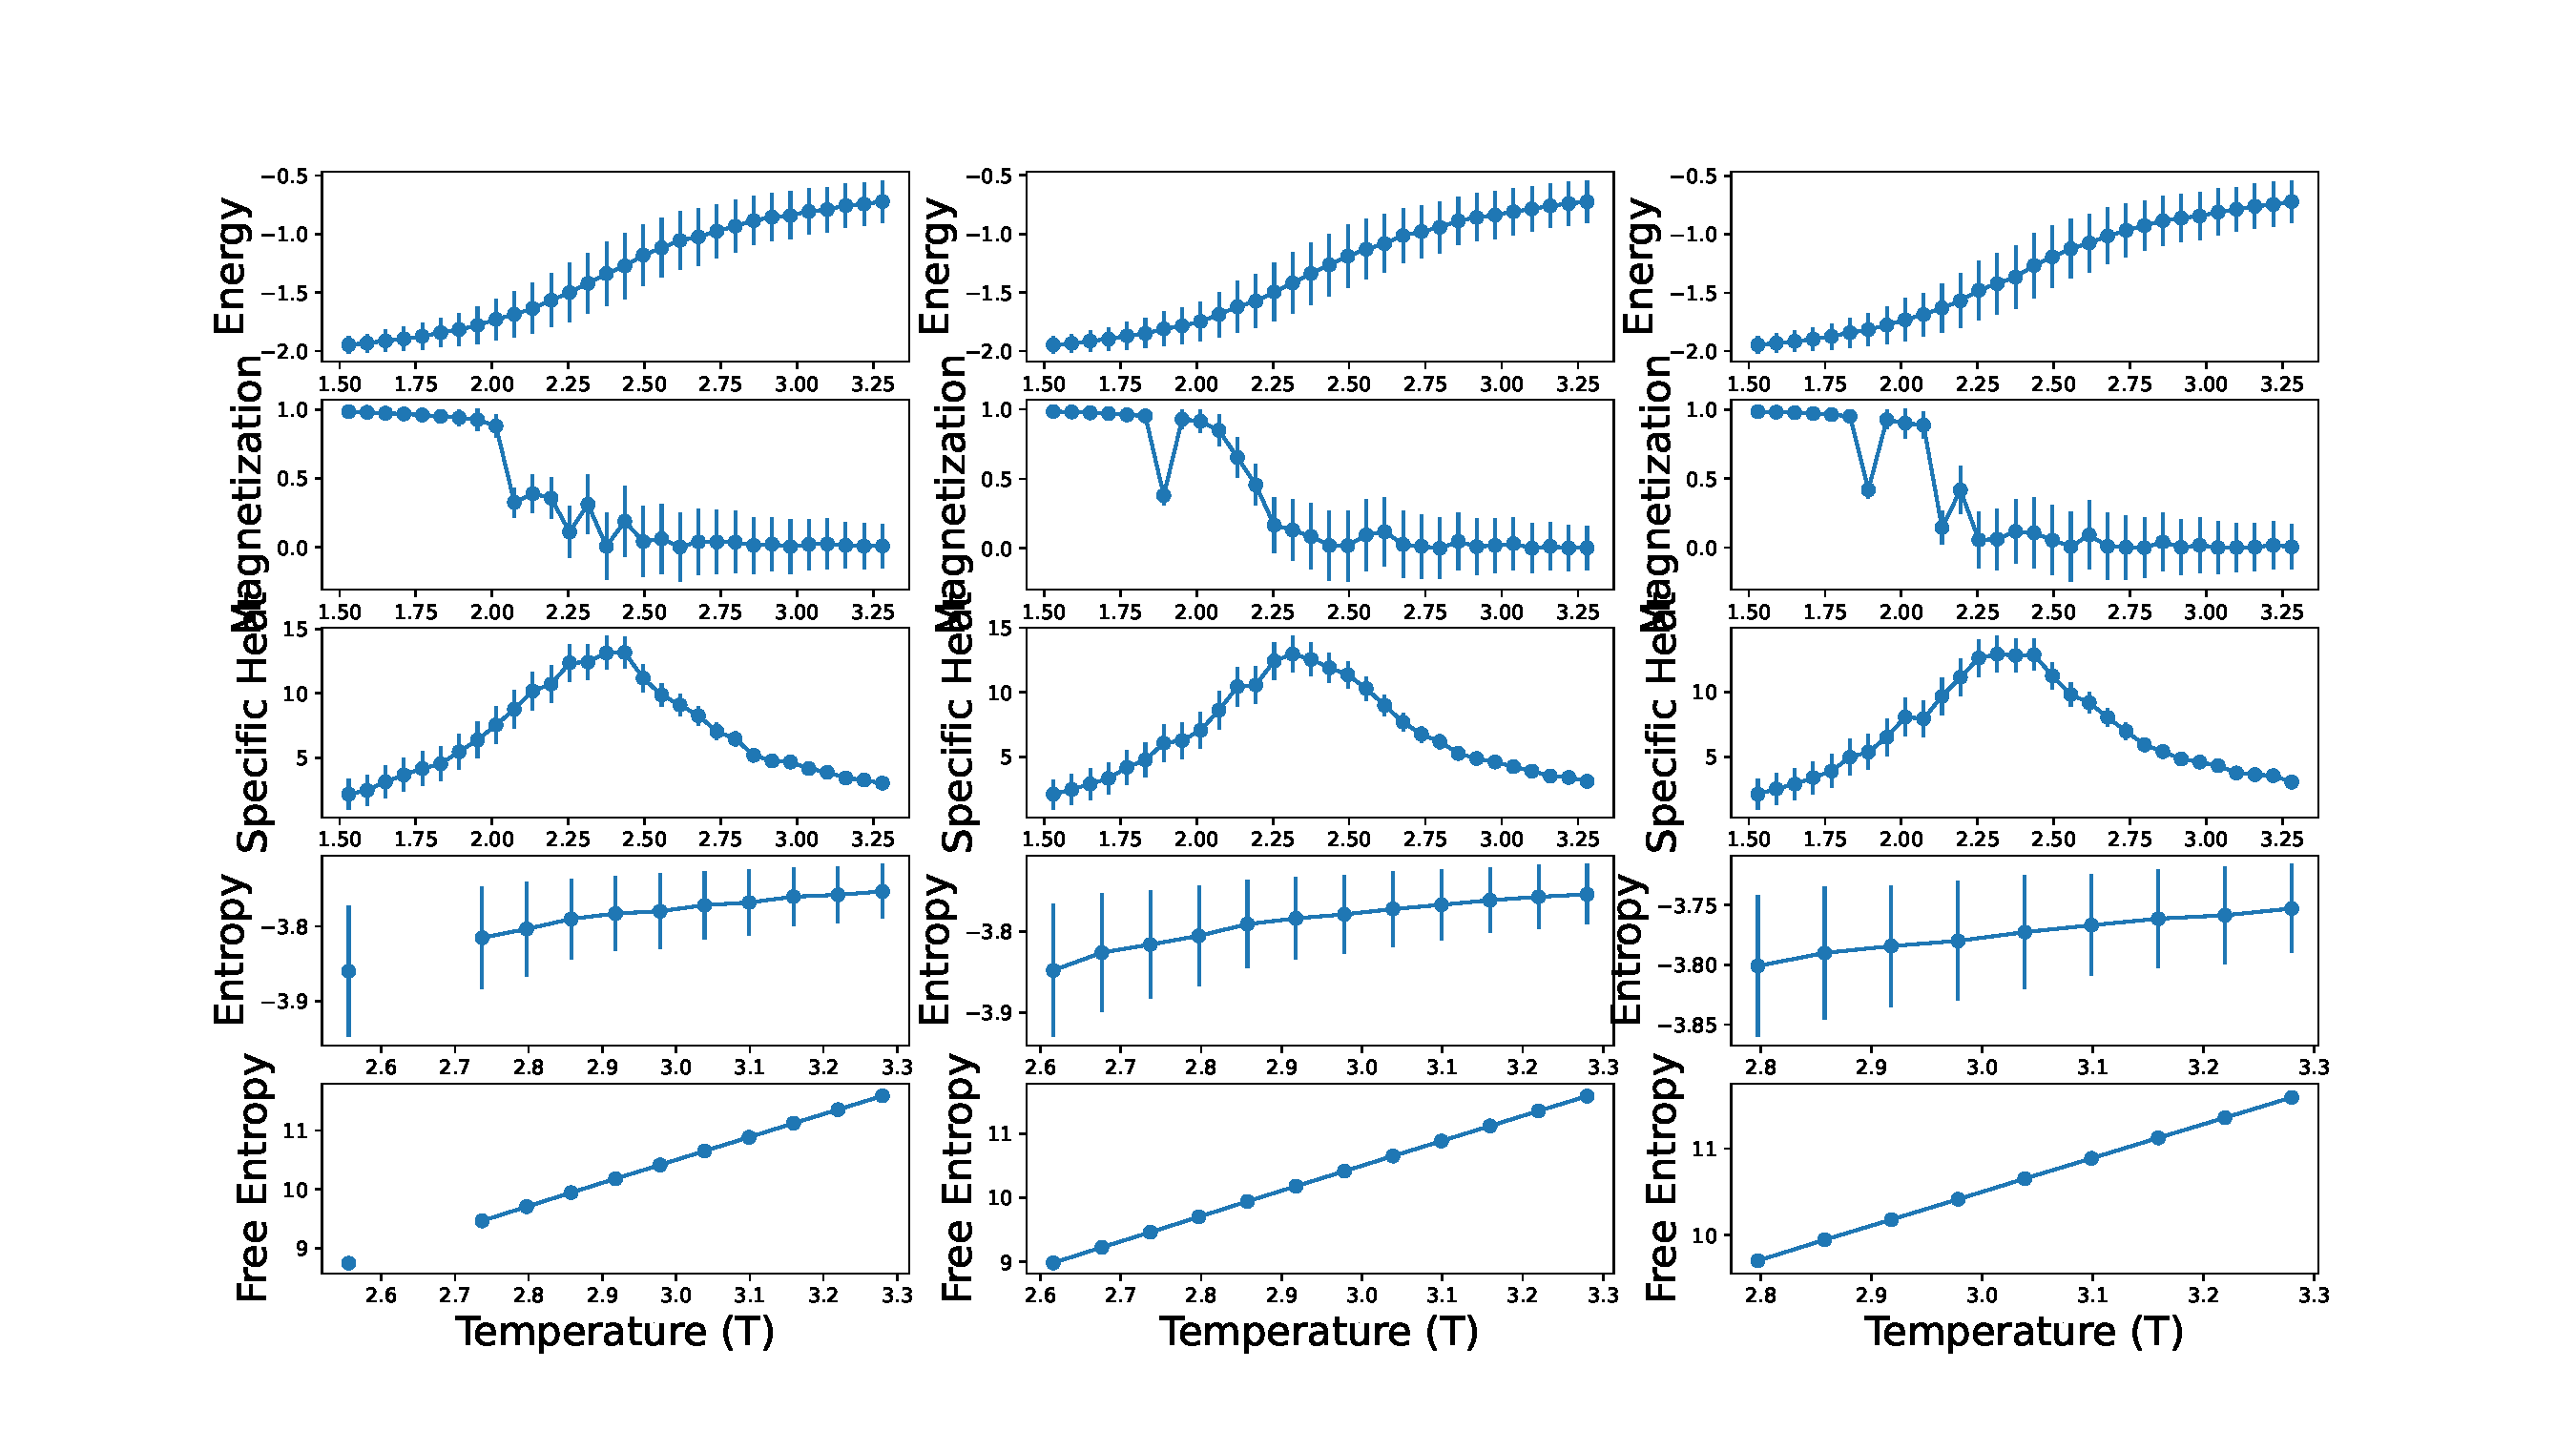
\includegraphics[width=0.8\textwidth]{pub/figures/q2c.pdf}
        \caption{The physical properties of the two-dimensional ising model %
            numerical simulations. We observed a sharp peak in the heat %
            capcity at the phase transition, which we used to estimate the %
            critical temperature of the simulation. From the heat capcity %
            we determined that the critical temperature was \(T_{c} = 2.25 \pm 
            0.02\) where our error corresponds to half the width of the %
            apparent peak. We noticed that the error in the measurements %
            was significant compared to their size particularly for the %
            heat capcity. This was most likely a result of the lower number %
            of that we used in the two-dimensional case. We were forced to %
            use more trials because of the increased compuational complexity.}
        \label{FIG5}
    \end{figure}

    \begin{multicols}{2}
        Given the partition function \(Z = (2\cosh(\epsilon / \tau))^{N}\), we 
        calculated the internal energy using,
        %
        \begin{align}
            U &= \tau^{2}\partial_{\tau}\ln(Z)\label{EQN1}\\
                &= \tau^{2}\partial_{\tau}
                    \ln\left(2\cosh\left(\frac{\epsilon}{\tau}\right)^{N}\right)
                    \nonumber \\
                &= N\tau^{2}\partial_{\tau}
                    \ln\left(2\cosh\left(\frac{\epsilon}{\tau}\right)\right)
                    \nonumber \\
                &= N\tau^{2}\partial_{\tau}
                    \left(2\cosh\left(\frac{\epsilon}{\tau}\right)\right)
                    \frac{1}{2\cosh\left(\frac{\epsilon}{\tau}\right)}
                    \nonumber \\
                &= N\tau^{2}\partial_{\tau}\left(\frac{\epsilon}{\tau}\right)
                    \frac{\sinh\left(\frac{\epsilon}{\tau}\right)}
                    {\cosh\left(\frac{\epsilon}{\tau}\right)}\nonumber \\
                &= -\epsilon N\tanh\left(\frac{\epsilon}{\tau}\right)
                    \label{EQN2}.
        \end{align}
        %
        We calculated the free energy of the system using,
        %
        \begin{align}
            F &= -\tau\ln Z \label{EQN3}\\
                &= -\tau\ln\left(\left(
                    2\cosh\left(\frac{\epsilon}{\tau}\right)\right)^{N}\right) 
                    \nonumber \\
                &= -N\tau\ln\left(
                    2\cosh\left(\frac{\epsilon}{\tau}\right)\right) 
                    \nonumber \\
                &= -N\tau\ln\left(
                    \exp\left(\frac{\epsilon}{\tau}\right) + 
                    \exp\left(-\frac{\epsilon}{\tau}\right)\right) \nonumber \\
                &= -N\tau\ln\left(\exp\left(\frac{\epsilon}{\tau}\right)
                    \left(1 + \exp\left(-2\frac{\epsilon}{\tau}\right)\right)
                    \right)\nonumber \\
                &= -N\tau\ln\left(\exp\left(\frac{\epsilon}{\tau}\right)\right)
                    - N\tau\ln\left(1 + 
                    \exp\left(-2\frac{\epsilon}{\tau}\right)\right) \nonumber \\
                &= -N\epsilon - N\tau\ln\left(1 + 
                    \exp\left(-2\frac{\epsilon}{\tau}\right)\right)\label{EQN4}. 
        \end{align}
        %
        The entropy followed from the combination of Equation \ref{EQN4} and %
        Equation \ref{EQN2} using Equation \ref{EQN5},
        %
        \begin{align}
            \tau\sigma &= F - U \label{EQN5} \\
                &= -N\epsilon\tanh\left(\frac{\epsilon}{\tau}\right) + 
                    N\epsilon + N\tau\ln\left(1 + 
                    \exp\left(-2\frac{\epsilon}{\tau}\right)\right)\nonumber \\
            \sigma &= \frac{\epsilon}{\tau}\left(1 - 
                    \tanh\left(\frac{\epsilon}{\tau}\right)\right) +
                    \ln\left(1 + \exp\left(-2\frac{\epsilon}{\tau}\right)\right)
                    \label{EQN6}.
        \end{align} 
        %
        Finally, we determined the specific heat using Equation \ref{EQN7} %
        and Equation \ref{EQN2},
        %
        \begin{align}
            C &= \partial_{\tau}U\label{EQN7}\\
                &= \partial_{\tau}\left(-N\epsilon\tanh\left(
                    \frac{\epsilon}{\tau}\right)\right)\nonumber\\
                &= -N\epsilon\partial_{\tau}\left(\frac{\epsilon}{\tau}\right)
                    \frac{1}{\cosh^{2}\left(\frac{\epsilon}{\tau}\right)}
                    \nonumber\\
                &= \frac{N\epsilon^{2}}{\tau^{2}\cosh^{2}\left(
                    \frac{\epsilon}{\tau}\right)}\label{EQN8}.
        \end{align}    
        %
        Using our one-dimensional ising model we numerically validated these %
        relationships, shown in Figure \ref{FIG2}. Based on the energy and %
        our knowledge of thermodynamics we concluded that all of the spins %
        aligned at \(\tau = 0\). This is evident because the magnitdue of %
        the energy increases while the entropy approaches zero indicating %
        a unique ground state. At high temperatures the heat capcity becomes %
        very small indicating that the addition of more heat will not change %
        the internal energy very much, and as predicted by the second law of %
        thermodynamics it approaches zero at \(\tau = 0\). We also tested the %
        one-dimensional scenario for a phase shift, described in Figure %
        \ref{FIG3} and found that the one-dimensional case did not have a %
        phase shift.

        To calculate the error bars shown in Figure \ref{FIG2} we used the %
        variance of each parameter averaged over the runtime of the simulation %
        following a burn-in period. This burn-in period was chosen to be 1000, %
        since this provided enough time for each spin to be visited ten times %
        without taking too long. To improve our investigation we could have %
        produced plots of the parameters at each iteration and estimated the %
        required burn-in time by identify on the graphs when equilibrium was %
        reached. 
    
        We generalised this process to a two-dimensional ising simulation. %
        As we decreased the temperature we found that there was a point %
        where the net magnetisation shifted away from zero. This can somewhat %
        be seen in Figure \ref{FIG4}. By running many additional simulations %
        we were able to visually estimate that the critical temperature for %
        the spontaneous magnetisation was approximately \(T ~ 2.25K\). We %
        later confirmed this from the peak in the heat capacity as discussed %
        in the caption to Figure \ref{FIG5}. As in the one-dimensional %
        simulations we estimated the error in the physical parameters from %
        their variance over the duration of the simulation following a %
        burn-in period.To estimate the error in the heat capacity we needed %
        to take extra care and used,
        %
        \begin{align}
            \Delta c &= \left(\text{var}(\epsilon^{2}) + 
                2\text{var}(\epsilon)\right) / N^{2} / \tau^{2},
        \end{align}
        %
        where we have attempted error propagation through the alternate %
        formula for the variance, \(\text{var}(\epsilon) = 
        \langle\epsilon^{2}\rangle - \langle\epsilon\rangle^{2}\), using %
        the variance itself as the error estimate for the means. This seems %
        very meta and we are not confident that it is correct.
    \end{multicols}
\end{document}
